\subsection{Winston Cone Refurbishment}

Winston cones (WC) are used to collect light onto the PMT photo-cathodes after one reflection.
In the LTCC there are three kind of WCs:

\begin{enumerate}

\item Small
	\begin{enumerate}
		\item Height: 18 cm
		\item Radius at the top: 20 cm
		\item Radius at the bottom: 11 cm
		\item Material: 0.25-cm thick copper (electro-formed)
	\end{enumerate}

	\item Medium
	\begin{enumerate}
		\item Height: 22 cm
		\item Radius at the top: 20 cm
		\item Radius at the bottom: 11 cm
		\item Material: 0.5-cm thick plastic (vacuum pressed)
	\end{enumerate}

	\item Large
	\begin{enumerate}
		\item Height: 30 cm
		\item Radius at the top: 22 cm
		\item Radius at the bottom: 11 cm
		\item Material: 0.25-cm thick copper (electro-formed)
	\end{enumerate}
\end{enumerate}

\begin{figure}[!h]
	\centering
	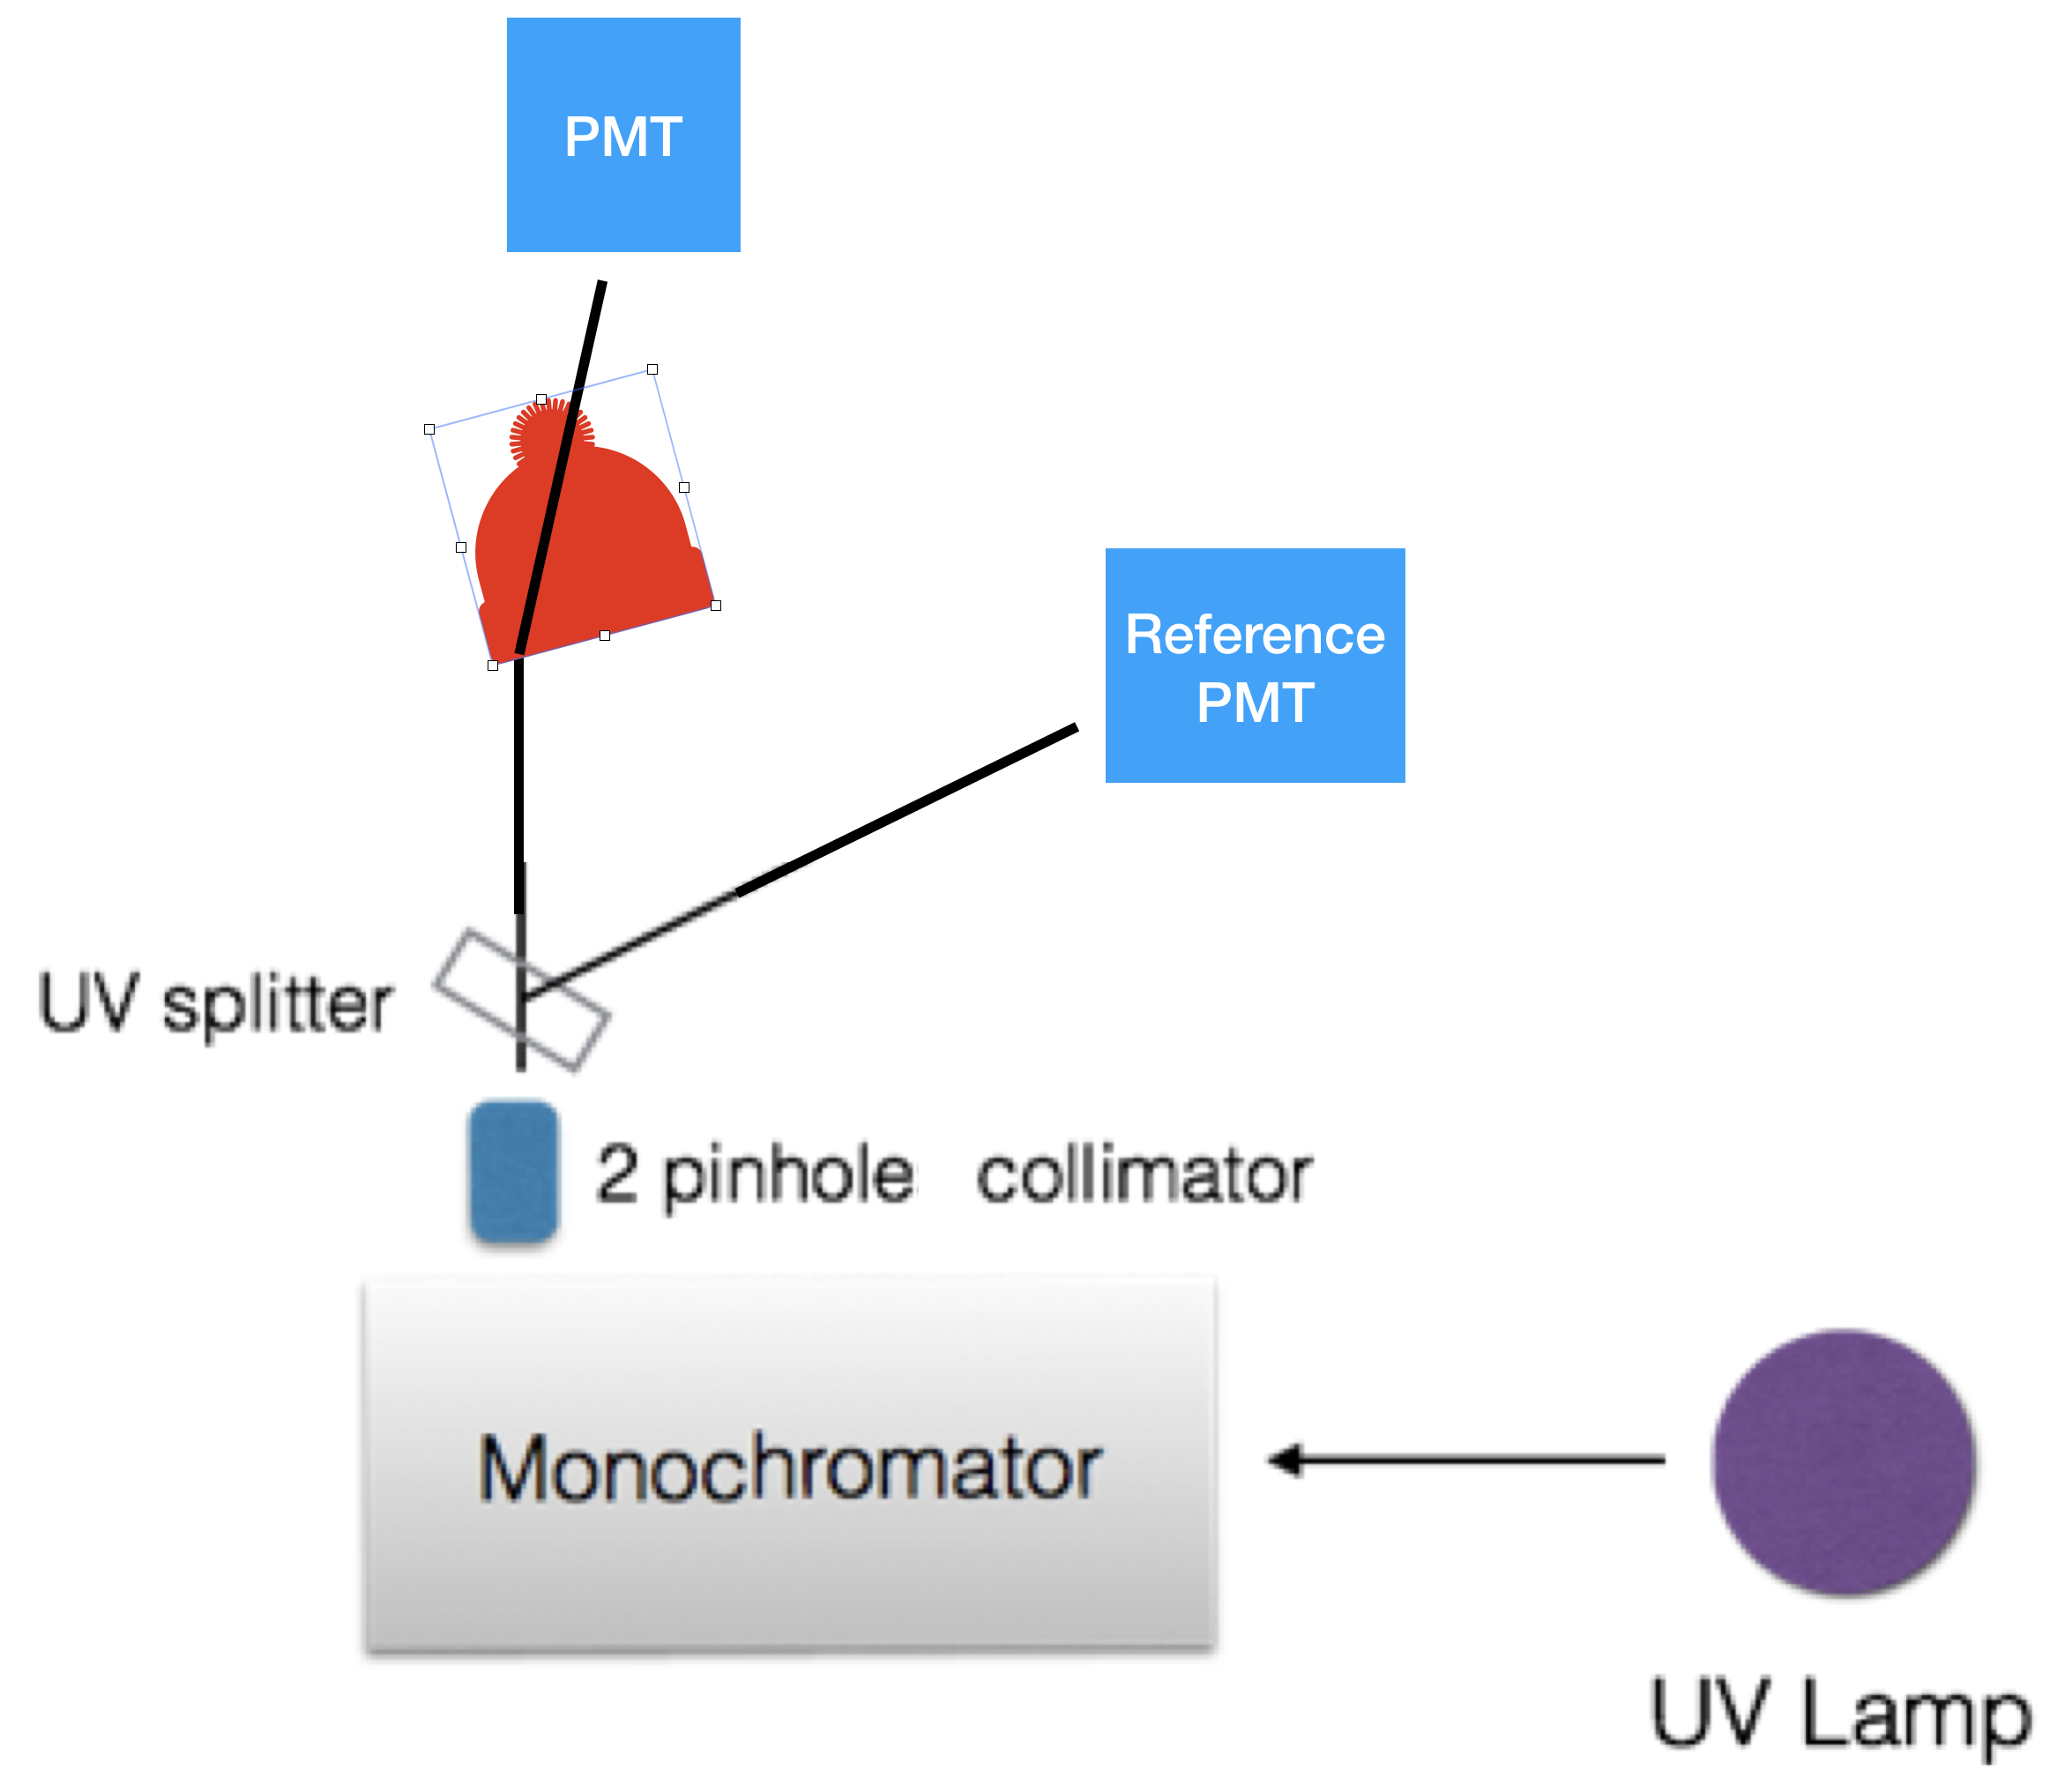
\includegraphics[width=0.98\columnwidth,keepaspectratio]{img/wcSetup.png}
	\caption{Setup to measure the WC reflectivity. The wavelength of light from a deuterium lamp was measured
          using a monochromator and split in two beams, each with calibrated intensity. One of the beams impinged on
          the WC at a typical angle of 12\mdeg, while the other was directed at a reference PMT. The reflectivity was
          measured in different spots for a sample of WCs.  The results proved to be independent of the spot location.}
	\label{fig:wcSetup}
\end{figure}

The reflectivity of the WCs showed quantitatively the same degradation as the mirrors. However, due to their shape,
re-coating of the WCs is more costly than the mirrors and the LTCC budget allowed refurbishing only 160 out of the
216 total WCs. A setup on an optical bench to measure the reflectivity for all of the WCs at wavelengths between 200
and 400~nm was designed to accept incident shallow angles of 10\mdeg-15\mdeg (typical incidence angle based on
simulation studies), see \F{wcSetup}. The typical reflectivity of a poor WC vs. wavelength is shown in \F{wcStatusBefore}
(top). All 216 WCs were studied, and the average reflectivity results are shown in \F{wcStatusBefore} (bottom). These
data allowed cataloging of the quality of the WCs to select the worst ones to refurbish. The cones were put in a vacuum
chamber and \coating\ was deposited on top of the existing coating. The typical reflectivity of a representative WC
after re-coating is shown in \F{wcStatusAfter} (top). About 30 cones needed the additional treatment of removing the
existing aluminum coating to improve the new \coating\ deposition. Even then, about half of these cones did not show
improvement probably because the treatment damaged their surfaces.
The results of the WC refurbishment are summarized in \F{wcStatusAfter} (bottom).

\begin{figure}[!ht]
	\centering
	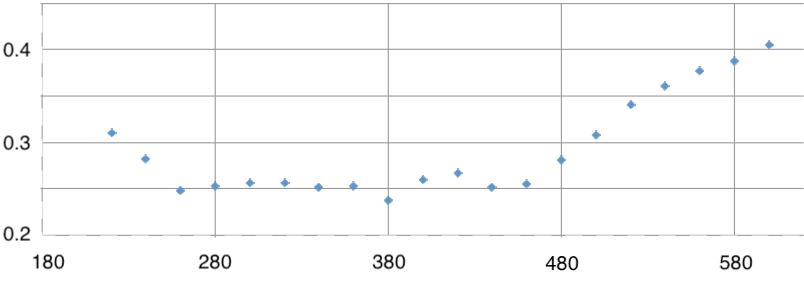
\includegraphics[width=0.98\columnwidth,keepaspectratio]{img/winstoConeSample2Reflectivity.png}
	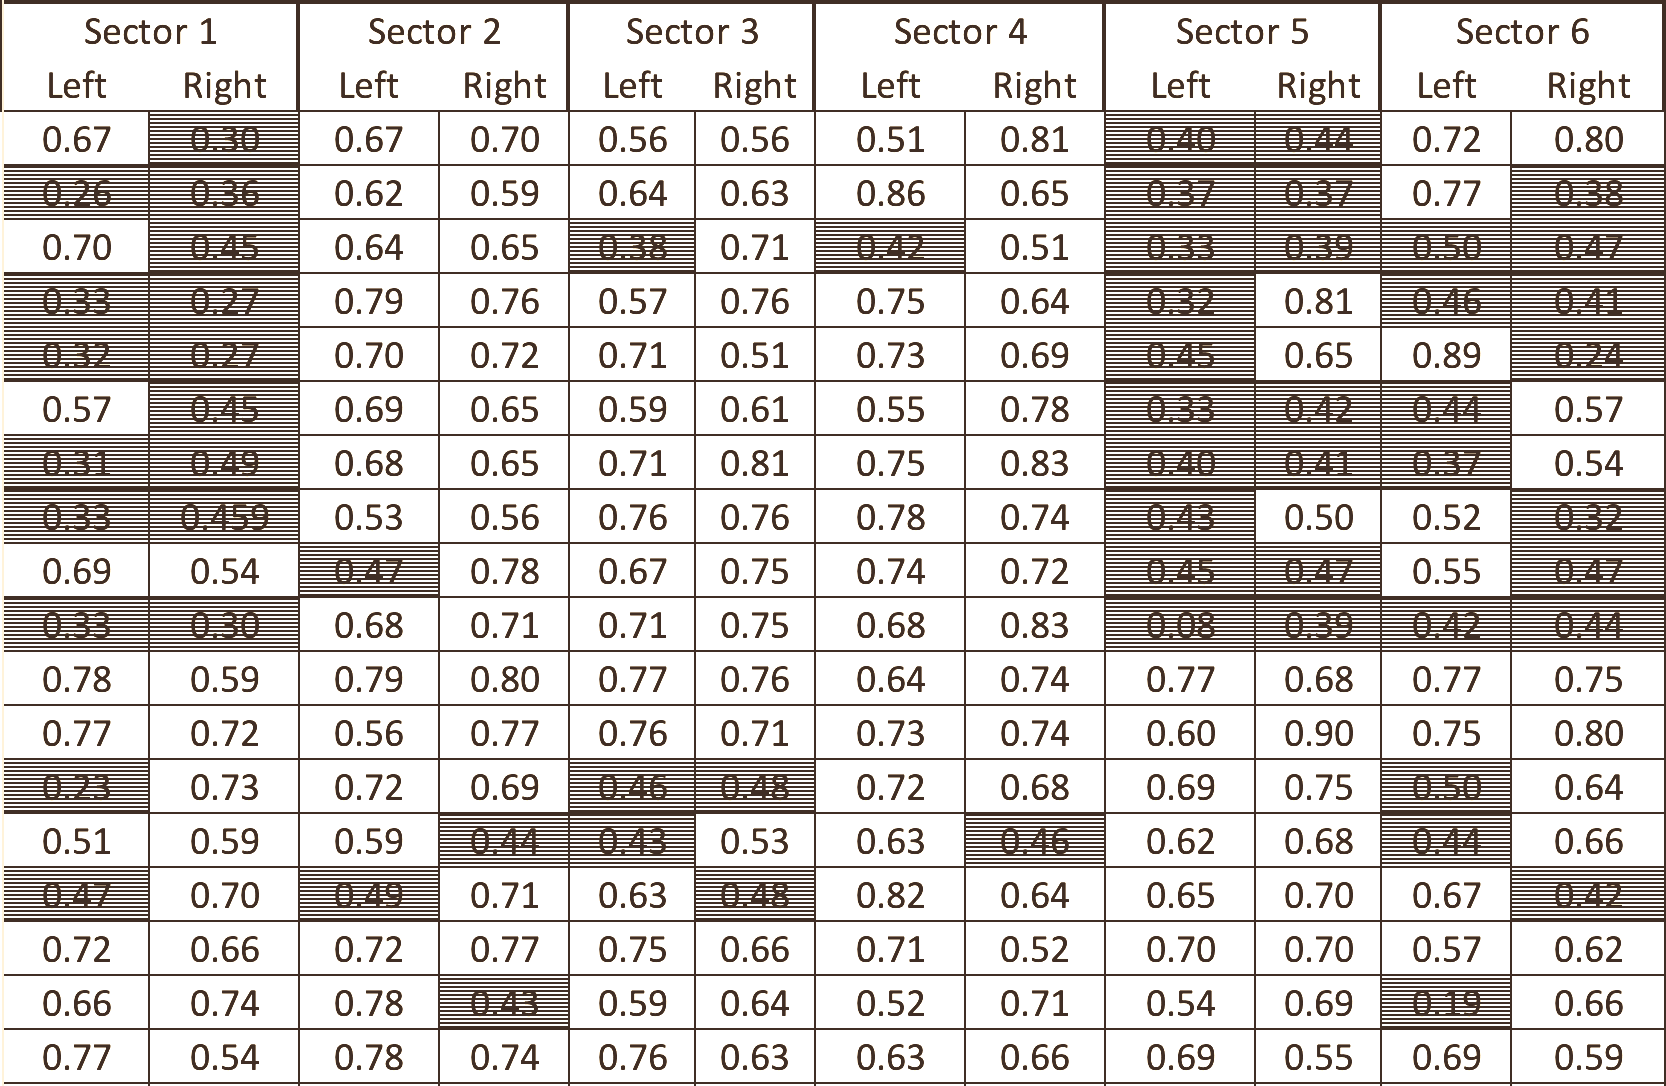
\includegraphics[width=0.98\columnwidth,keepaspectratio]{img/wcStatusBefore.png}
	\caption{Top: typical reflectivity vs. wavelength (nm) of a ``very poor'' WC. The reflectivity is below 30\% for
          most wavelengths between 200 and 400~nm. The reflectivity proved to be independent of the particular spot
          on the WC surface. Bottom: the average reflectivity $r$ between 200 and 400~nm for all WCs. The shaded
          gray boxes represents WCs with poor reflectivity ($r < 50$\%).}
	\label{fig:wcStatusBefore}
\end{figure}

\begin{figure}[ht]
	\centering
	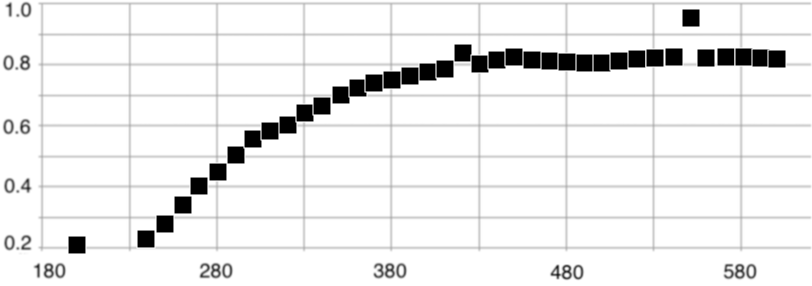
\includegraphics[width=0.98\columnwidth,keepaspectratio]{img/winstoConeSample1Reflectivity.png}
	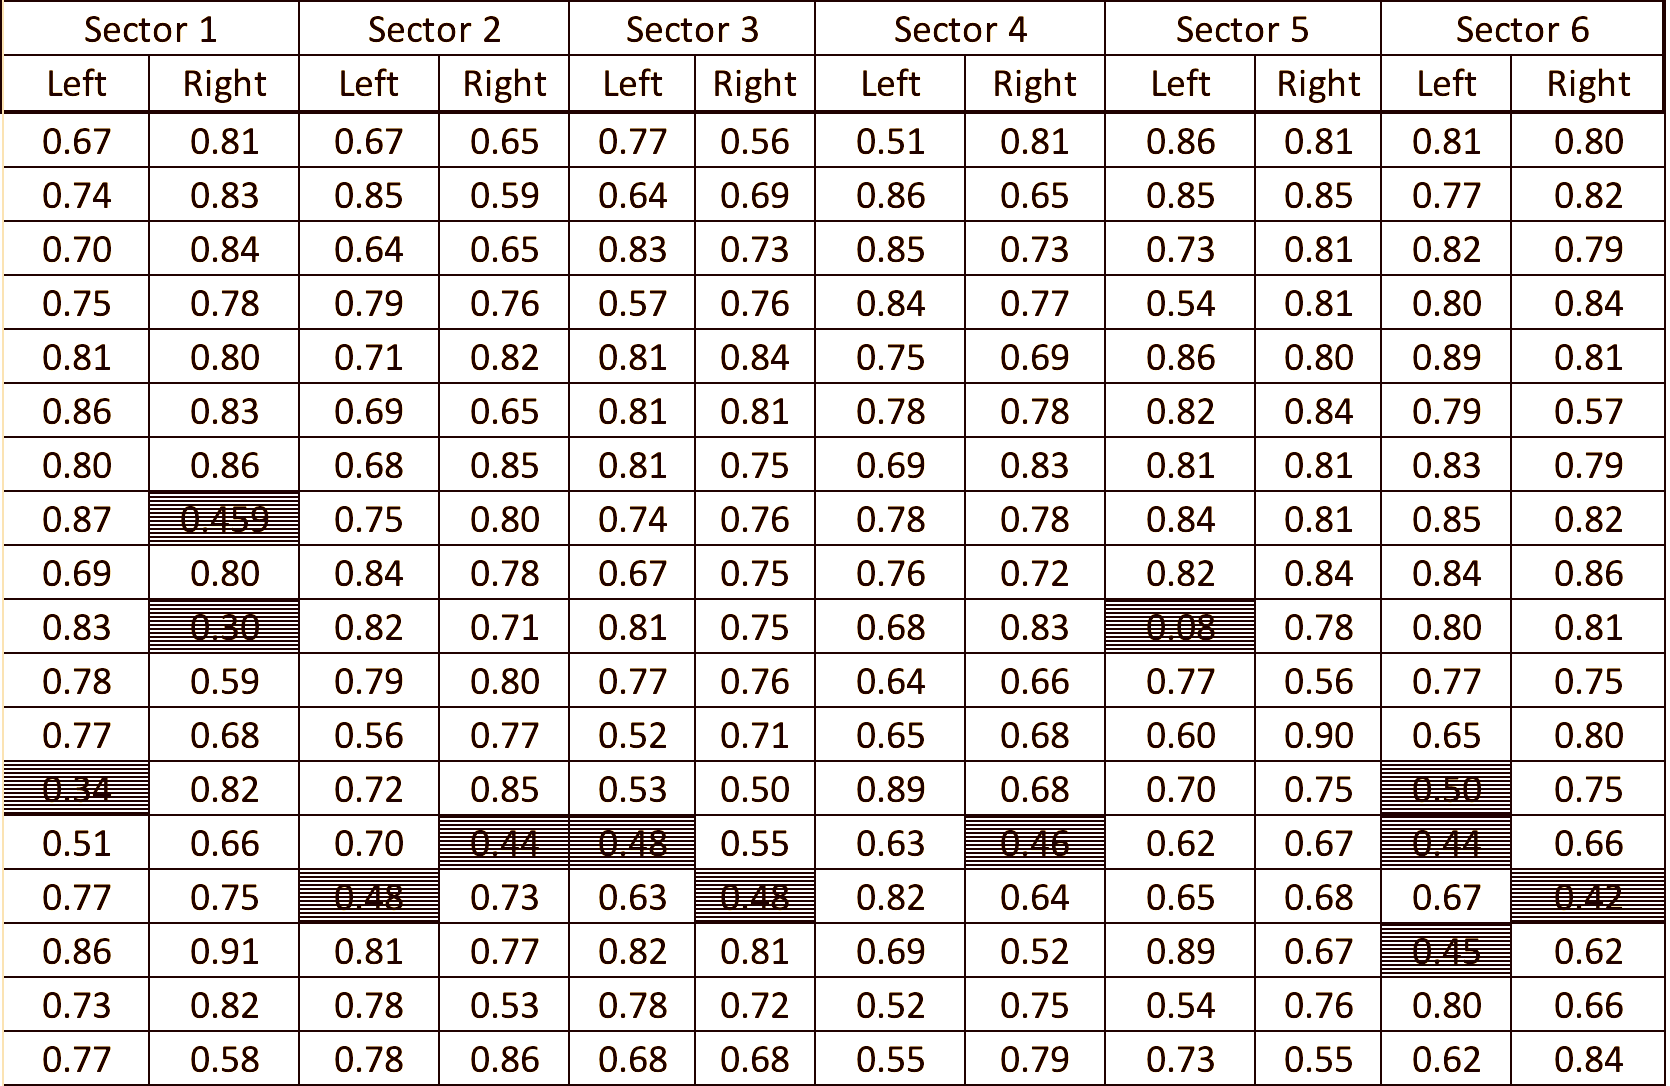
\includegraphics[width=0.98\columnwidth,keepaspectratio]{img/wcStatusAfter.png}
	\caption{Top: typical reflectivity vs. wavelength (nm) of a ``very poor'' WC after refurbishment. The
          reflectivity quickly rises to 65\% at a wavelength of about 340~nm. Bottom: average WC reflectivity $r$
          between 200 and 400~nm for all WCs. The shaded gray boxes represents WCs with poor reflectivity
          ($r < 50$\%). This picture should be compared to \F{wcStatusBefore}. Most re-coated WCs show improved
          reflectivity.}
	\label{fig:wcStatusAfter}
\end{figure}
